\chapter{Исследовательская часть}

\section{Среда для тестирования}

Для тестирования разработанного алгоритма применялась облачная платформа Google Colab, не требующая установки ПО на локальный компьютер.

\begin{lstlisting}[label=lst:2,caption=Отчёт по результатам классификации]
	              precision    recall  f1-score   support
	
	Ham       				 0.96      1.00      0.98       966
	Spam       				 0.99      0.74      0.85       149
	
	accuracy                           	   0.97      1115
	macro avg       	 0.98      0.87      0.92      1115
	weighted avg       0.97      0.97      0.96      1115
	
	@Дополнительные метрики@:
	MCC: 0.8421
\end{lstlisting}

\begin{figure}
	\begin{center}
		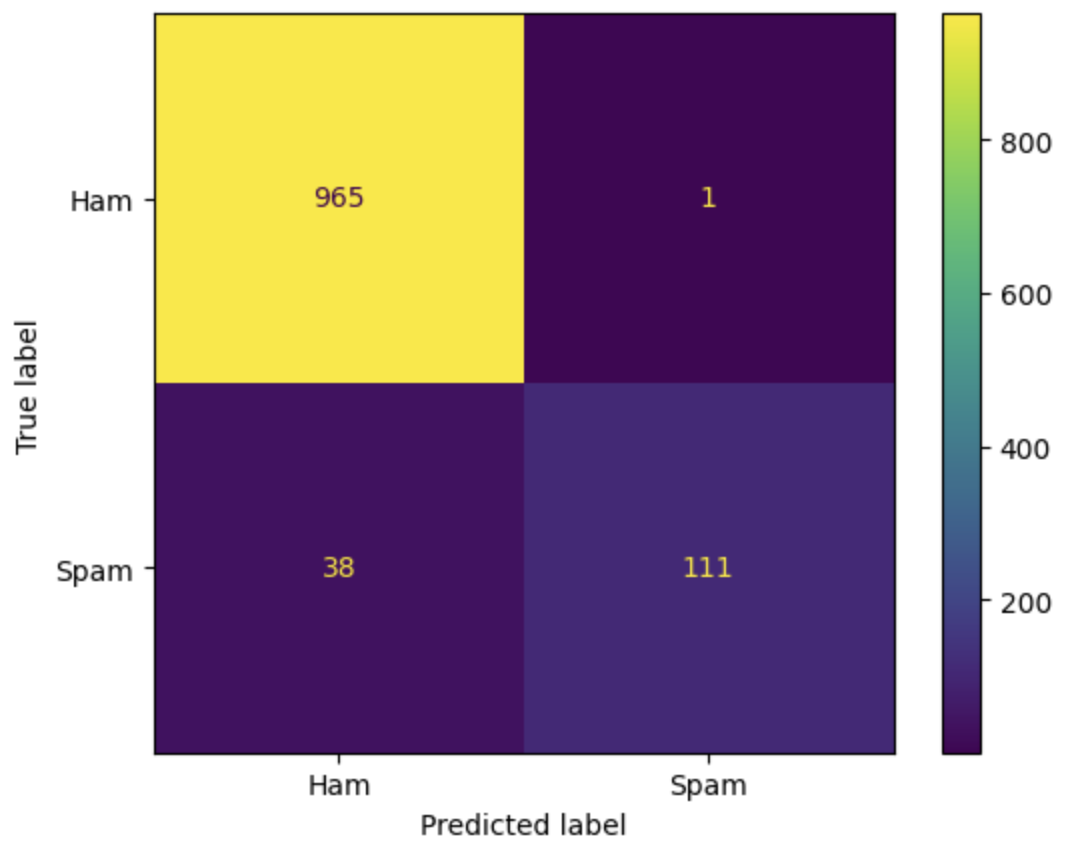
\includegraphics[width=\textwidth]{images/1.png}
	\end{center}
	\caption{Матрица ошибок}
	\label{img:1}
\end{figure}

\begin{figure}
	\begin{center}
		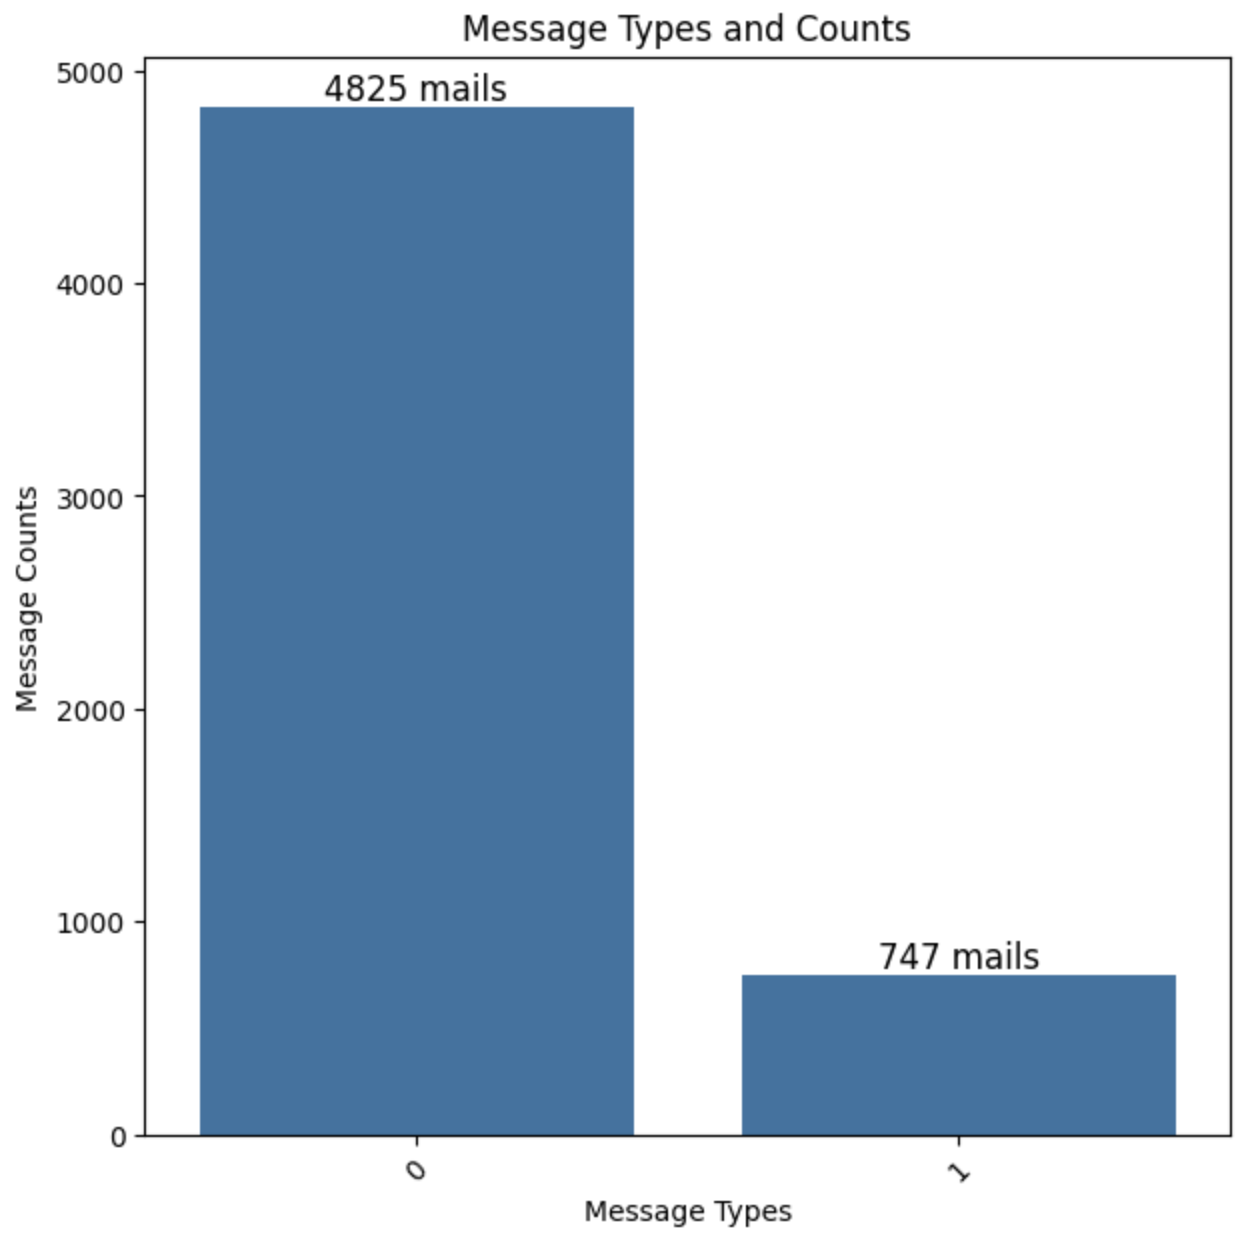
\includegraphics[width=\textwidth]{images/2.png}
	\end{center}
	\caption{Соотношение размеров классов}
	\label{img:2}
\end{figure}

\begin{figure}
	\begin{center}
		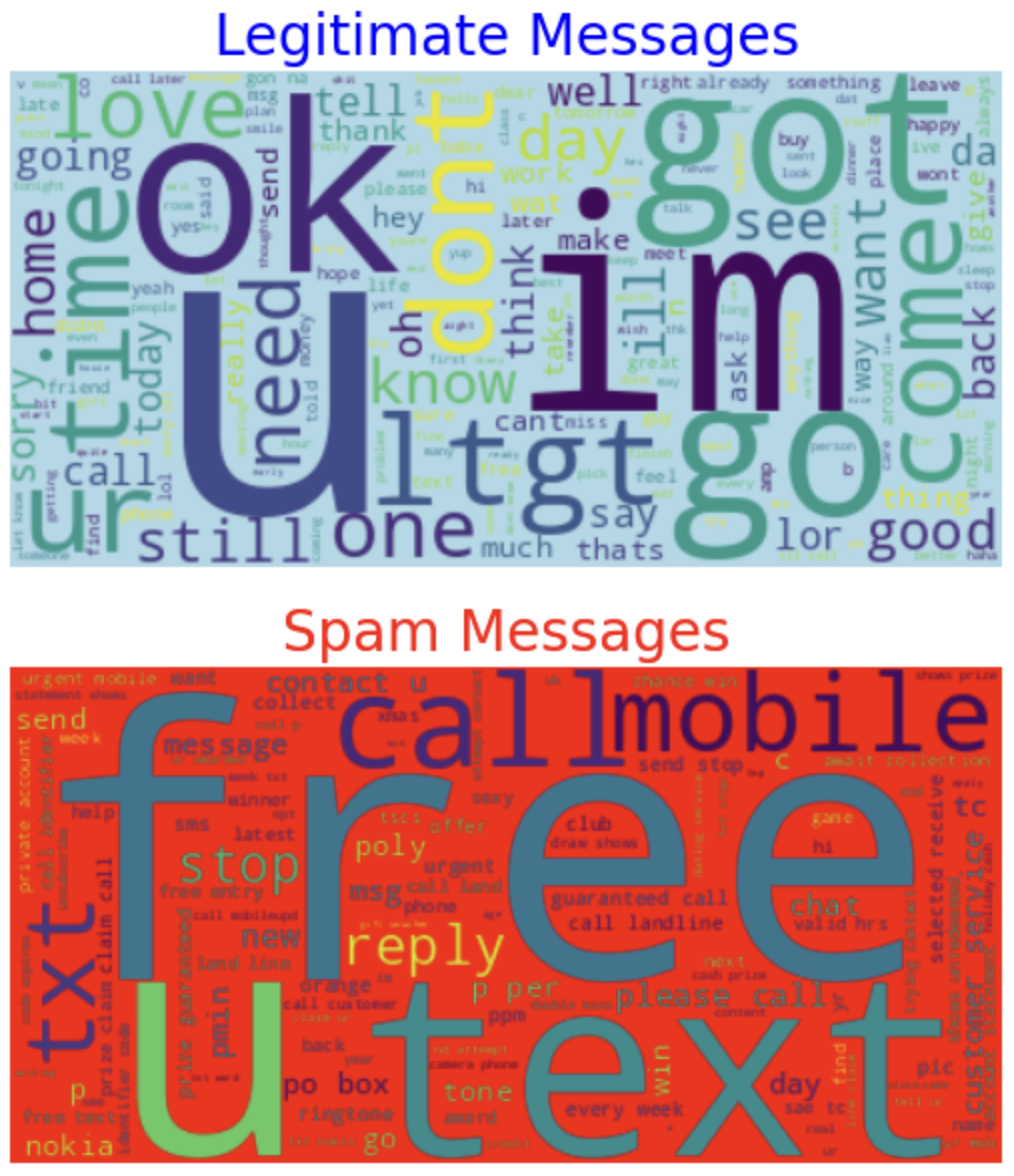
\includegraphics[width=\textwidth]{images/3.png}
	\end{center}
	\caption{Наиболее часто встречающиеся слова для каждого класса}
	\label{img:3}
\end{figure}

\clearpage
